\documentclass[a4paper, 11pt]{article}
\usepackage[T1]{fontenc}
\usepackage[utf8]{inputenc}
%\usepackage{margins}
\usepackage[bottom=2.8cm, nohead]{geometry}
\usepackage{palatino, url, multicol}
\usepackage{amssymb, graphicx, fancyhdr, latexsym, url, verbatim}
\usepackage{algorithm, algorithmic}
\usepackage{hyperref}
%\usepackage{natbib}
\usepackage[all]{xy}
\usepackage{listings}
\usepackage{cite}
\usepackage{float}
\usepackage{makeidx}
\usepackage[english]{babel}
\usepackage[font=small,format=plain,labelfont=bf,up,textfont=it,up]{caption}
\usepackage{xspace}
%\usepackage{subfigure} % has to be loaded after caption to prevent clash Commented, because subfig is the newer (and presumably
% better) version of subfigure...
\usepackage{subfig}
\usepackage{xcolor}	
%\usepackage[titles,subfigure]{tocloft}
%
%
%\setlength{\cftbeforesecskip}{0.1cm}
\newcommand{\todo}[1]{\colorbox{red}{\color{white}#1}}
\newcommand{\projectName}{Bachelor Thesis - Flood Simulation Browser\xspace}
% xspace only puts a space where we want one!

\addtolength{\headheight}{-05mm}
\addtolength{\headsep}{05mm}

\pagestyle{fancy}
\lhead{\projectName}
\rhead{\small F.S.B.}
%\cfoot{\footnotesize \textit{ \projectAbbreviation}\\[0.1cm] \small \thepage}
%\cfoot{}
%\rfoot{\thepage}

\lstset{
	tabsize=2, 
}
\setlength{\parindent}{0pt}
\setlength{\parskip}{10pt}

\begin{document}
\newcommand{\HRule}{\rule{\linewidth}{0.5mm}}

\begin{titlepage}
\begin{center}

\includegraphics[width=1\textwidth]{uva}\\[0.5cm]

\HRule \\[0.2cm]
{ \huge \LARGE \textbf{\projectName}\\[0.1cm]
 \vspace{0.2cm}}
\HRule \\[0.4cm]
\Large \today

\vfill

\begin{tabular}{ll}
	\textbf{Supervisor:}  & 	\textbf{Executive:}  \\
	Robert Belleman  - U.v.A &  Richard Torenvliet \\
	& stdnmr: 6138861 \\ 
	R.G.Belleman@uva.nl & Richard.Torenvliet@student.uva.nl
\end{tabular}
\end{center}
\end{titlepage}
%\thispagestyle{empty}
\newpage
\tableofcontents
\newpage

\begin{abstract}
In this thesis we discuss the design and implementation of a cross platform application, designed specifically for tablets, that assists the UrbanFlood project in making simulated flood more accessible for viewing simulations. This application for viewing simulated floods was already available on a multi-touch table, which is not easily transportable. To reach to goal of mobility, and to reach a larger audience, it is desirable to have a more portable instrument. As tablets have the same interaction features as the multi-touch table, they are the ultimate tool to achieve this goal. Sencha Touch 2 was found to be the best option at first to build a cross-platform application, but a more in-depth study showed that it could not fully live up to the expectations. A second objective of the present study is to test how many clients can be handled by the back end server at ones. Tests show that the response time goes up considerably with the number of users, which shows that there are also server side problems to be solved before widely applying the developed software.
\end{abstract}

%\documentclass[10pt,a4paper]{article}
%\usepackage[utf8]{inputenc}
%\usepackage{amsmath}
%\usepackage{amsfonts}
%\usepackage{amssymb}
%\usepackage{listings}
%\usepackage{graphicx}
%\author{Richard Torenvliet - 6138861}
%\title{Flood Simulation Browser}
%\maketitle

\section{Introduction}
The UrbanFlood is a European project that aims to create an early warning system in European cities\cite{UrbanFlood}. In the today's changing climate, more and more cities have to deal with floods more often. \todo{Boek ref}. Due to extreme rainfall, rising water or long lasting drought, the instruments that protect the civilians of a certain area are negatively influenced. The project involves setting up a system that can make estimates on how dikes would behave in the near future. Vigilance against weak spots in the dykes is needed 24/7. To do this they placed sensors in dykes that can be monitored remotely via internet. But this not the only concern. They also developed a system that can create flood simulations of a certain area. This is used for testing dikes in a possible scenario but also for educative proposes. This subjec is discussed in the present document.

This project concerns the Flood Simulation Browser. The concept of this browser is to illustrate/visualize a flood in a particular area. With this technology people can see the flow that the water will take. When a dike breaks it is important to know where the water will flow. Information about which locations in the area will be under water first can result in a successful evacuation plan. This system already exists, but is build for a multi-touch table only and is accessible by few people. The project that is the subject of this thesis, aims on making it easier available and accessible. The accessibility of the application (the tablet can be at night stand of the dijkgraaf) makes it more likely that someone with right authority can take better decisions about placing/reinforcing dikes or creating evacuation plans. Moreover, if this system is more accessible, then civilians of a certain neighbourhood that is threatened by water, have the ability to gain knowledge of where the water will go first. They then are able to take the the right crucial decisions based on this knowledge in the hour of need.

The implementation will be on a multi-touch device. In particular iPad\cite{ipad} and Android\cite{android} tablets. Users can use this application in an intuitive way to get more intelligence about the complex situation at hand. They have the ability to choose from several simulations that were already made for a specific area and also creating new simulations.
This thesis covers design choices that where made in order to reach that goal. The first step is to get an idea of the existing simulation system of which this application will make use of. This includes a description of where this application is situated in the Urban Flood Project as a whole. The study also includes an extensive examination of the capabilities of the different devices available, as well as a requirement analysis specifically for this application. The resulting app will be intend to extend the simulation with a use-ability and above all mobility factor. Of course, performance is one of the main issues here. 

A second objective of this study is testing the scalability of the REST\todo{ref REST} server. By testing how much requests the server can handle at once it helps the urban flood project to estimate how many users can use the application simultaneously. The original multi touch application on the multi touch table was only one client for the server. It's important to know that an early warning system stays online under the heavy load of a multitude of clients.

The scientific research of this project will be devoted to the development of an intuitive design. The main research will be, where do buttons, lists, and other important components need to be situated in the application. Another aspect of this project is the research for scalability of the server. This data will provide information about how many users can be handled by a server at once. The important part of this research will be the decision making of which framework or tool to use for the implementation of this application.

The first part of this document will describe the global information needed for the second part of this document. The division into parts is made along conceptual lines. The first part contains specific/technical information. The ones that only care about the global information are served by the first part and the ones that are interested in how this application came to be are served in the second part of this document. Note that an understanding for how this application was made, the information of both parts are needed.

\part{Discovering the subject}
\label{part:Discovering}
\section{Flood Simulation System}
Two systems are involved in creating the backbone and resource for the Flood Simulation Browser(F.S.B). One part is the system where the client application directly communicates to and where the API is stalled. The other is used by that system to simulate new simulations when a request at client side is made. The systems are needed for retrieving data about a simulation and ultimately to display the simulations. This generation of new simulations is a service of HR Wallingford \cite{wallingford}, a company specialized in providing services like these for water management projects. The F.S.B. is a GUI\cite{GUI} that can display the simulations on a map that were made by the HR Wallingford's server and retrieved from\url{sangkil.science.uva.nl}.

The simulation system of HR Wallingsford runs in the cloud. That means it does all the calculation for the client and it is not important to know at which physical computer the simulation runs. The system can calculate simulations by providing parameters about a certain area. For instance, the location and how much water you want to simulate. When a simulation is submitted and calculated, the simulation is stored. With http calls(GET or POST) to the API at \url{sangkil}, it returns a set of simulations that are present. The important thing to note is that the simulation consists of images that have to be displayed on a map, e.g. Google Maps. The flood simulation system performs a complex simulation with the height map of the area. The height map holds detailed information about the height of an area. With this data, the flow of the water can be calculated and turned in to images. These images are used by the client application, this an important part of this project.
Not only does the system calculates the flow of water but it also calculates the estimated route that people take. It can calculate how much people would survive a simulated flood, keeping in mind that this project is all about saving people, this is interesting information.
 
\subsection{Flood API}
The F.S.B. needs an API as a resource of data. Without resource the F.S.B. has no meaning. Therefore the an API already exists on \url{sangkil.science.uva.nl}.

The API is a REST API \cite{REST} that returns a JSON \cite{JSON} formatted string when data is requested. The API functions as an interface to get the data of simulations and to start new simulations. It's a client server system where requests are done by the client and the appropriate data is transferred back to the client. With this data, information about a certain simulation can be displayed. The data can be in the form of an image or information in .csv \cite{CSV} files. The .csv files can be plotted and displayed in a chart. See part two for more information about the returned payloads.
As previously described, new simulations are not done on the same server but are done by HR Wallingford. They provide a service to do such simulations. The API will run new simulations at HR Wallingford when the client requests them, the new simulation will appear in the in the list of simulations available on by the API. In short, the F.S.B. doesn't do anything directly with the simulation service of HR Wallingford.

\section{Flood Simulation App}
\subsection{Platform considerations}
\subsubsection{Mobile Website}
As stated in the introduction the application is meant for tablets, but not specifically for iOS or Android. Which means cross-platform. How to maintain the cross-platform demand on the application is one of the subjects of this project. This means that the application is not a native implementation and consists of one code-base and runs on more devices. There is a tool called PhoneGap \cite{PhoneGap} that uses HTML5\cite{HTML5}, CSS3\cite{C3} and Javascript to build the app. In essence the developer builds a mobile website and PhoneGap can wrap this in an application. The native web-engine is used to render the mobile website. PhoneGap can result in a huge speed-up in development time, which is a huge advantage. The speed up can be obtained by the fact that previously gained skills of webdevelopment can be re-used. Therefore there is no need to learn a new programming language or sdk\cite{SDK} for native apps. For example Objective C for iOS and Java for Android. The disadvantage can be that the application feels more like a mobile website than a real app. In addition, the end product depends on the support of today's web-standards. Not all browsers have full support for HTML5 and CSS3, which forms the bases of a successful implementation of the application. For a list of supported elements, websites like caniuse.com \cite{CSS3} can be used to determine the percentage of support for a certain element/feature. But that does not really help. Nevertheless, the lack of the native feel oan application can be remedied. For example, frameworks where native-like elements are created for you while coding in a programming language already known by a webdeveloper also exist.

\subsubsection*{Native Elements}
This solution is Titanium Mobile, the Appcelerator \cite{Titanium-Appcelerator}. Titanium Mobile can build mobile applications that are in fact native applications. By programming in Javascript and call functions to create native elements the application can be created. The framework builds semi-native code, unlike the previously discussed PhoneGap. The development for this platform is fast and an application for both iOS and Android are quickly off the ground. But there is also a disadvantage to using Titanium. The applications are big, around 11MB no matter what. Because of the fact that the logic will still be in javascript(compiled), Titanium has to ship their javascript engine to the device. But not only do Titanium generated apps take a lot of space, it also has trouble with memory, see this blog-post\cite{memoryleak}. The blog-post discusses this issue, both developers and users discuss this issue in the reactions. Although this blog post refers to version 1.6 and 2.0 is already out, we consider the uncertainty about this behaviour of Titanium too great a risk for the present project.

Moreover developing and testing on iOS provides expected behaviour and a large part of native elements are supported. For Android the native elements are mostly \textbf{not} the elements you thought they would look like. To reach cross-platform apps, the developer needs to constantly keep track if they're building an element for iOS or for Android. It might be stated that the functionalities of different platforms are not evenly supported. iOS is by far the most supported platform. This only provides an advantage if the project only meant to run on iOS. The idea of Titanium Mobile is great, it works fine but will delay developing time when you truly want to reach crossplatform. Also the fact that this application needs a map that supports overlays for the simulation images is a big disadvantage. By searching trough the documentation \footnote{\url{http://docs.appcelerator.com/titanium/2.1/index.html\#!/api/Titanium.Map}}, the only thing it supports is adding an annotation. An annotation is just a marker placed on the map with the ability to get de latitude and longitude of the marker. To sum up, Titanium lacks support for both platform and map object, at the same time it can surprise the developer in an unpleasant way by taking a lot storage and a buggy garbage collection.

Building crossplatform and creating native elements could mean a risk for completing the application. A browser is the only thing that has the most equality on both devices, i.e. both Android's and iOS's native browsers are based on the webkit engine\cite{webkit}. Webkit is an open source web engine that is used by both Safari and Chrome.
\subsubsection*{Javascipt frameworks}
As already explained, PhoneGap only provides the possibility to create an app out of a website. This website can be built in any way the developer likes, using web technologies supported on the native device. There are frameworks that can speed up the development to make an intuitive application. Two frameworks that are considered are: jQuery Mobile \cite{jQuery-Mobile} and  Sencha Touch \cite{sencha}. 
\begin{description}
\item [jQuery Mobile]
This Javascript framework is build out of one Javascript file and one CSS file that the developer includes. By giving certain HTML elements a data attribute, which is a HTML5 element, the framework uses this to create views. A page is made by declaring a div adding data-role="page". Such a page can be given a footer like div data-role="footer". 
Switching frame one page to the other can be as simple as giving a html anchor a href to an id of a page. Figure \ref{fig:jquery} provides an example that will result in two pages. Both pages have a button. Both buttons link to the other page (foo, bar), so tapping on one button will change the page to the other page.
\begin{figure}[H]
\begin{lstlisting}
<div data-role="page" id='bar'>
	<a #href='foo' data-role="button">switch to foo</a>
</div>
<div data-role='page' id='foo'>
	<a #href='bar' data-role="button">switch to bar</a>
</div>
\end{lstlisting}
\caption{jQuery Mobile, pages example}
\label{fig:jquery}
\end{figure}

Creating two pages is quickly done, the downside of jQuery mobile is that in order to create an application where views look alike, you have to repeat yourself. You have to create pages with other id's and with the same look/elements but with different information. The conclusion for jQuery mobile is that it is easy and the developer does indeed use HTML5, CSS3 to create views.  But it is not easy to built a modular application. It is always possible to create such a modular application yourself, but when creating an application which is not such a framework the developer will run in to creating a framework in stead of the intended application.

\item [Sencha Touch 2]
Sencha touch 2 is a framework focused on the Model View Controller design pattern \cite{MVC}. It encourages the developer to use this pattern. The way of developing really differs from jQuery mobile. Where jQuery mobile sets you free to do whatever you like, Sencha Touch constraints the developer using components that are available in Sencha Touch. The difference can be easily explained with an example.

In the items array, see Figure \ref{fig:sencha}, the items in that array can be anything supported by Sencha Touch like lists, a tabview, a map, etcetera. 

Sencha Touch provides a command-line tool to build a starting environment. It creates files where the developer can start from. It is recommended to use this as a starting point. The advantage is an application that is structured out of the box with a design pattern that is the current standard(MVC). With Sencha Touch 2 there is no need for PhoneGap, unlike jQuery Mobile. Sencha Touch 2 provides the possibility to run the code on your simulator or native device with the command line tool. Testing for Android and iOS became much more simple, resulting in less developing time. Running PhoneGap for Android, needs Eclipse\cite{eclipse} to build, for iOS the developer needs to build in Xcode\cite{xcode}. When testing on both devices the developer needs to be able to test in both environments, and testing from the command-line is a lot easier than running both environments. 

A disadvantage of Sencha Touch could be, as seen in figure ~\ref{fig:sencha}, the syntax of Sencha Touch is not so easy at first. So the learning curve could be very steep.
The last argument that has a great influence on deciding which framework to use, could be that Sencha Touch provides an add-on that has the capability to create multi-touch charts. The original implementation of the urban flood browser on the multi-touch table has this feature. It would be a great extension of the project if this was possible. So with an eye on the future it could save a lot trouble, and it could add up to a more intuitive design. The next section will discuss this in more detail.

\begin{figure}[H]
\begin{lstlisting}
Ext.application({
    name: 'foo',

    launch: function() {
        Ext.create("Ext.tab.Panel", {
            fullscreen: true,
            items: [
                {
                    title: 'bar',
                    iconCls: 'bar',
                    html: 'bar'
                }
            ]
        });
    }
});
\end{lstlisting}
\caption{Sencha Touch application example. This example creates an application with the name 'foo'.  The html can be placed inside the items array. }
\label{fig:sencha}
\end{figure}
\end{description}

\subsection{Requirements Analysis}
\label{sec:requirements}
Requirement analysis for this project is an inventory making of tasks that the application has to be able to perform. I.e., the requirements on the application, as opposed to the requirements that the application needs to run. These requirements are as follows. First, the users need to be able to see different simulations and be able to distinguish where certain simulations are located. By starting with displaying the locations that are available would be the starting point where the users can start interacting with the application. For displaying the locations, a request to server is needed to for displaying those. 
The locations are mostly named by cities. The corresponding simulations have to be retrieved from the server and displayed in a list. Those list-items are the individual simulations, so it makes sense that when tapping on a list item, the simulation of the related item is going to be displayed. The form of these simulations are important. The simulations are in the form of images. These images are images from above and can be placed on the map. In order to display these images, there has to be a map available. Next, the data of where to place the image is needed for creating a map. This data is located in the simulation data of the city. In part two of this document the exact implementation can be found.

The flood simulations are in the form of multiple imagery that is placed on the map. A requirement for these simulation images is that the user can control which image it wants to see in a chronological way, of course the user does not decide what the sequence is going to be. This requirement results in the need for controls. These controls need to be displayed somewhere in the viewport when the user has tapped on a list item of a simulation.

The flood simulations contain information about how much cubic meters of water is present in a certain timestep in a specific location. The simulations are divided in zones and labelled with an id. So a simulation contains information, this information needs to be displayed in such a way that it can be interpreted by the user. This would require a chart of some sort with the timesteps on the x-axis and some other value like volume on the y-axis. To determine the zone which contains the information, a latitude and longitude information is needed again. How this is done is described in part 2 of this document.

\subsection{App Design} 
\label{sec:appdesign}
The application will be used on tablets so that a lot of space can be used. On tablets the screen is larger than on mobile phones. Which can result in a bigger travel distance of the user's hands. The GUI design has to be built with the considerations of the interaction capability of the users. For instance, unlike with mobile phones, according to Clark(2012) a leading designer in creating multi-touch applications, people tend to hold a tablet on the top halve of the tablet when holding with both hands, Figure \ref{fig:perimeter}. The focus of the user is going from top to bottom. The top elements of the application will draw the first attention of the user. That's why Clark(2012) advises to place the important controls on the top half of the screen. The components that are important have to be placed in the left or right top of the screen, concerning the perimeter of the thumbs, Figure \ref{fig:perimeter}. The F.S.B.'s design heeds Clark's advice.
\begin{figure}[H]
\center
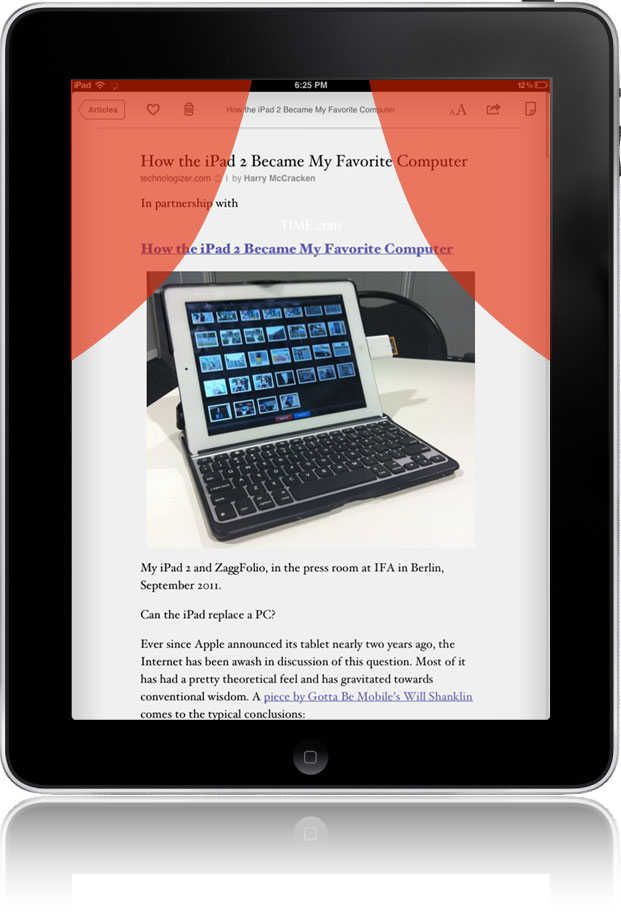
\includegraphics[scale=0.3]{touch.png}
\caption{Portrait touch perimeter(Clark, 2012)}
\label{fig:perimeter}
\end{figure}
First of all the flood simulations are done within different cities. This can typically be a list of cities. The list is scrollable and can be seen as an "infinite" array of cities around the world. Every city has it's own array of simulations to show. It therefore makes sense to also show these in a list. When a city is selected, the user has no use of the capability to select other cities and it's simulations. That's why the list of cities are pushed out of the viewport and the list of simulations is pushed in. 
It also makes sense to have one Map object in the view, where one city (latitude, longitude) can be shown at a time. The map object is the most important component of the browser. Inspired by Clark(2012) it can be stated that a hierarchy in importance of different view components can result in a different place on the screen. By placing the Map component always in the view and also as the biggest component, the idea of placing objects in a hierarchy of importance in the view is kept in mind. For an example of this, see Figure \ref{fig:mockup}.
The list component where cities and simulations are placed is at the left side of the view. It could also be the right side but it would not matter. Since two hands are more or less symmetrical, so placing the list object left or right would not be a problem. It does matter concerning controls. Controls to change the timestep of a simulation are definitely needed. A simulation consists of multiple images on different time steps. By giving the user control of which image is seen at which time step is a crucial feature in the browser. Since the list is placed in on the left side of the screen the controls appear on the right side of the screen, in the right top part of the screen. That way the perimeter of the thumbs are concerned.
\begin{figure}[H]
\center
\begin{tabular}{c}
	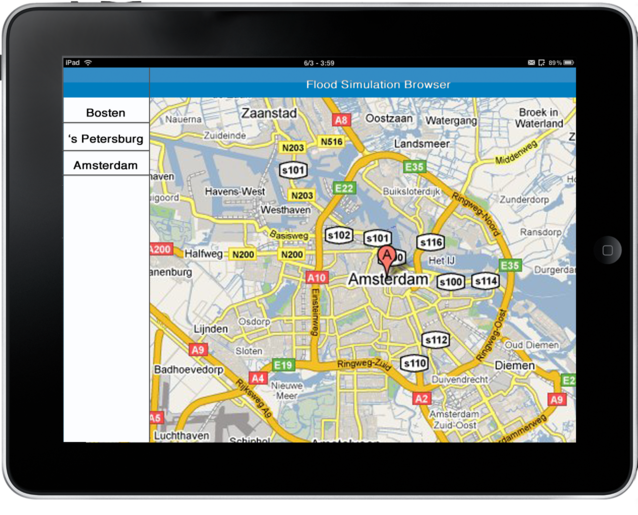
\includegraphics[scale=0.3]{mockup1_1.png} \\
	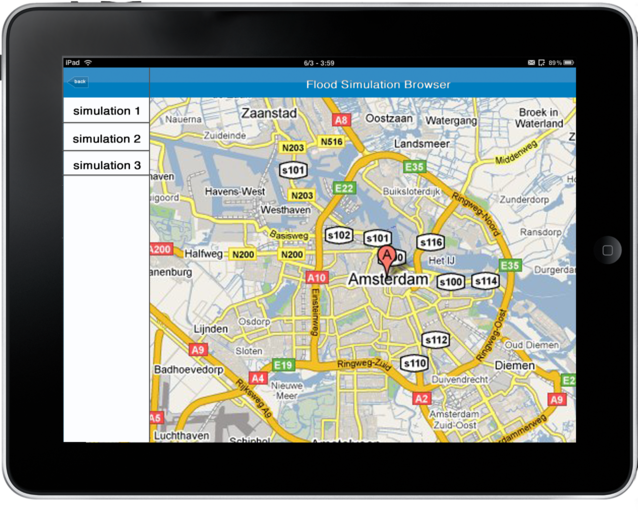
\includegraphics[scale=0.3]{mockup2_1.png}
\end{tabular}
\caption{Cities list of which simulations are available}
\label{fig:mockup}
\end{figure}

The flood simulation browser that is already built for the multi-touch table has the ability to submit new simulations to be simulated in the cloud. The spot of the simulation can be arbitrary on the map, by simply touching a place on the map and alter some parameters, the cloud service can create a new simulation to be seen. Although this feature can be an seen as an extension of my project, with time left this feature can be build in. That's why it can be considered in the App's design. The controls of these parameters need to be somewhere in view, by placing this in the neighbourhood where the user touches the map could be intuitive. However this should never happen when  the user is just navigating over the map, the user has to know that if he or she is the mode of with picking a place where to create a new simulation. 

Furthermore, it's an important feature to display data of a simulation in certain area. The API provides this data. It holds information about how much water flows in that area over time. This data is the volume of water per time step. The API requests latitude, longitude values, it then returns data of a location that is closest to this point. The application needs to display this data in a clear and understandable way. Charts are great way to display this data. In development of this application there needs to be a clear understanding of what usability is. Only displaying a chart of certain values could not be enough to learn anything or draw conclusions about the flood. The goal is to make use of the Sencha Touch Chart framework in order to provide comprehensive data of a flood in a certain area. See Figure \label{fig:senchachart} for an example of the chart framework.

\begin{figure}[H]
\center
	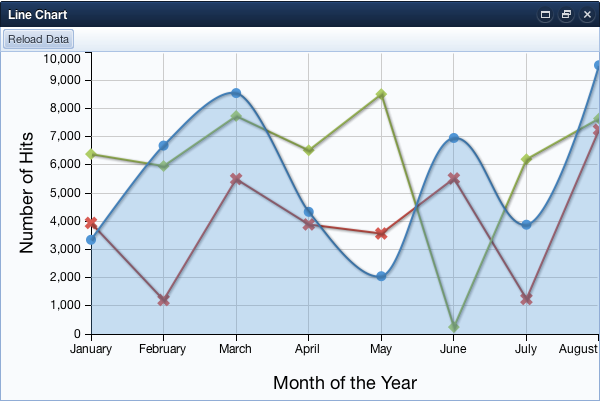
\includegraphics[scale=0.5]{chart.png} \\
\caption{Example of sencha chart}
\label{fig:senchachart}
\end{figure}

\subsection{Scalability}
\label{sec:scalability}
The second assignment of this thesis is to test the scalability of the server. The server address is \url{sangkil.science.uva.nl}. To test this server it is required to exclude any other parameter of the client. Such as maximum download speed, maximum throughput, latency of the network. The idea is not to test this at a home pc, but test it in a server that is hooked up in the same network as \url{sangkil.science.uva.nl}. More specifically, the connection between \url{mangkus.science.uva.nl}(hosted at the same location as sangkil) and \url{sangkil.science.uva.nl}. If this is the case the exclusion of restricted variables at client side could be possible. 
For stress testing the server a tool called siege \cite{Siege} would be of assistance. With this tool it is possible to launch requests to a url with $n$-nodes and $k$-connections executed per second. Siege registers the following data:
\begin{itemize}
\item Transactions - total hits
\item Availability - percentage of total succeeded hits
\item Elapsed Time - seconds
\item Data Transferred - MB
\item Response Time - seconds
\item Transaction Rate - $\frac{Transactions}{Elapsed Time}$
\item Throughput - MB/s
\item Concurrency - rate of concurrency
\item Succesful transaction - number of succeeded hits
\item Failed transactions - number of failed hits
\item Longest transaction - seconds
\item Shortest transaction - seconds
\end{itemize}
With this data new insight can be provided. By increasing the number of simultaneous connections, values could start to change. To really give the server a stress test, it is possible to provide a list of urls which can randomly be picked and executed. This simulates a more likely scenario and provides more insight on how the server would behave in a real situation. The expectation is that the response time might grow as the number of clients starts to grow. With more clients to serve, it could take longer if there are more clients active. If processor power is limited, maximum available memory is reached or even the implementation of the server for handling requests could all have an effect in the response time, or any other variable. The research for which variables changes, together with the cause and the solution is a part of this project and will be documented in the end report. 


%\section{Conclusion}
%The project will be implemented with the framework Sencha Touch 2. All encountered issues will be discussed in the end report. This %nformation can be used in future projects relating to creating cross-platform applications. Also all data about the scalability of the erver %will be documented. The urban flood project can in turn use this data in future plans to invest in more server power. If they do not need %to invest in more power this is also important.
%This project will ultimately result in a cross-platform application that can be used by the public or government to gain information %about a certain area.

\section*{End of Part one}
Part \ref{part:Discovering} describes the questions and some answers on what the approach of tackling this problem is going to be. For an understanding of what global problems are faced in this project, it will be sufficient to have read part one. Part \ref{part:implementation} holds information about how the implementation is made, the problems that where discovered in process, results are displayed and discussed and ultimately ending with the conclusion of this project. 

\part{Implementation Details}
\label{part:implementation}
\section{Server API}
A clear understanding of which request have to be done in order to gain the right information is needed first before beginning with any implementation. The full api is referenced in the appendix \ref{appendixA}. The appendix is referenced and used for explanations in the following sections.

\section{Sencha Touch 2}
The final choice for the development of this application was made in favor of Sencha Touch 2.  Sencha Touch provides cross-platform capability and is based on web technology. Although Sencha Touch comes with a unique syntax, based on Ext (reference!!), the content, look and logic is based on web languages.
Part \ref{part:Discovering} section \ref{sec:appdesign} the design of a touch application is discussed. The application is going to be created with the findings described in that section. Also the mockups in Figure \ref{fig:mockup} created early on in the project are great for keeping track on what the end goal should look like. 
%The requirements of the application discussed in section \ref{sec:requirements} are created in 

Sencha Touch is based on MVC with the addition of stores. Stores can hold information of whatever the application needs, more about this in a moment. The model is used for the communication with the database, the controller stands between the model and the view. The controller can steer between views and handle logic. The application has no direct need of models, since there is no database that has to be updated. Stores can handle enough communication between the server and the application. 

\subsection{Stores and Lists}
The stores in this application are prominently used for filling the lists. In particular the cities list en \texttt{simulationslist}. A list object is defined as the follows.

\begin{figure}[H]
\begin{lstlisting}
store = Ext.create('Ext.data.Store'{
    fields: ['name', 'corners', 'visbounds', 'area_id', 'center', 'size'],
	proxy: {
			type: 'rest',
			url: 'http://sangkil.science.uva.nl:8003/area/list.json',
			reader: {
				type: 'json',
				rootProperty: 'areas'
			},
		}
});
Ext.create('Ext.List', {
	title: 'locations',
	store: 'citystore',
	itemTpl: '<div>{name}</div>',
});
\end{lstlisting}
\caption{List of cities}
\label{fig:sencha}
\end{figure}
The store is automatically updated when the values change on the server. When something changes in the store, the list is also automatically updated. The specified fields are available in the list, containing the name of the field between brackets \texttt{\{ \}}, the field name of record $n$ is placed in list item $n$. Five stores are present in the application. \texttt{SimulationStore.js}, \texttt{SimulationDetailStore.js}, \texttt{LsmStore.js}, \texttt{SimulationsSummary.js}, \texttt{ChartStore.js}. 
\begin{itemize}
\item SimulationStore.js \\
Is sync with \url{http://sangkil.science.uva.nl:8003/area/list.json} on the server. Locally the store is in sync with the view \texttt{List.js}. Basically this store returns information of the simulation locations that are available. The most important data are the name, center, visbounds and area\_id. With the name for displaying in the list-item; the center for changing the map's center to the location of the simulation and the visbounds are used for the image overlay. When the user taps on a location, the data of longitude and latitude information is used to change the center of the map and push a new list over the current list, since a tap event on a list-item returns the tapped item and the store used for creating this list. The second list holds information about which all the simulations available.
\item FloodDetailStore.js \\
Is in sync with multiple urls, \url{http://sangkil.science.uva.nl:8003/area/<area\_id>/info.json}, where the area is the area that is selected in List.js. This store adds information of dikes. The rest of the data is already present in the SimulationStore.js. The dikes consists of eight values, which are 4 corners with a latitude and longitude value. This means that a polygon can be formed from these four locations and displayed on the map.
\item LsmDetailStore.js \\
This store holds information of the population dynamics, meaning how the evacuation of the individuals will proceed. 
\item SimulationSummary.js \\
Syncs with \url{http://sangkil.science.uva.nl:8003/drfsm/list.json?summary}. This returns a json string that holds a list of all the simulations.Luckily a store can be filtered on a certain value. All the simulations have an area\_id specified. The store is filtered on the area\_id selected in List.js. Note that filters stay present, so before doing anything the store has to be cleared of all the filters.
\item ChartStore.js \\
This store is used for creating the chart. The chart expects a jsonStore with data and fields to plot. The data is retrieved from the server at run time of the application in \texttt{Api.js} and set in the store by the setData function.
\end{itemize}
\subsection{Layouts and xtype}
Layouts in sencha touch provide a structure for placing components and are fairly easy to create. A layout keyword is placed in the Container component which functions as a container for other components. That way the developer can build a hierarchical view. Child components are placed in the items key array. These can be any component the developer likes. A layout in this application is used ones in \url{app/view/main.js}. 

\begin{figure}[H]
\center
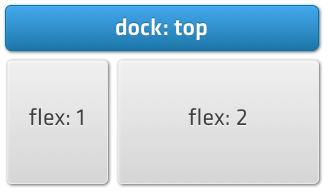
\includegraphics[scale=1]{ui/docktop.png}
\caption{layout with hbox}
\label{fig:layout}
\end{figure}

Next to the type layout hbox also vbox exists, which divides the viewport vertically.  The xtype keyword tells sencha touch which component to place in the container. Flex 1 or flex 2 tells the container on which side of the container the components needs to situated. See \ref{fig:layout_impl} for how these are used to as a reference. The image of figure \ref{fig:layout} is implemented in figure \ref{fig:layout_impl}.

\begin{figure}[H]
\begin{lstlisting}
Ext.define("app.view.Main", {
    extend: 'Ext.Container',
    config: {
        title: "Simulation Browser",
        layout: "hbox",
        fullscreen: true,
        items: [
        {
            xtype: 'listpanel',
            flex: 1,
        },
        {    
            xtype: 'simulationpanel',
            flex: 2
        }],
    }
});
\end{lstlisting}
\caption{Layout in \texttt{app/view/Main.js}}
\label{fig:layout_impl}
\end{figure}
The xtype keyword matches the keyword out of the component where the xtype is defined. It serves as shortcut to the full component. Components that are created can get a unique xtype value and be referred to by other components to call functions or for displaying  of that component, this is widely used throughout the application.
 

\subsection{Controllers}
Controllers preform the logic in the application. They react on events, fired by the elements in the view. In sencha touch the events are configured in the control configuration. References to components in the view are created in the ref attribute in the config attribute. A reference may consist of a css selector or an xtype name, or both. References are used in the functions below the config field, \texttt{this.getMap()}. Controllers are declared like the following.
\begin{lstlisting}
Ext.define('app.controller.Main', {
	extend: 'Ext.app.Controller',
	config: {
		refs: {  
			map : Map      
		}
		
		control:{
			#button: {
				tap: tappedButton
			}
		}        
   }   
	tappedButton: function(){
		this.getMap().dofunction();
	}
});
\end{lstlisting}
In the application two controllers exists, a \texttt{app/controller/main.js} controller for handling logic for the general view and simulations. Another controller named \\
\texttt{app/controller/chartController.js} is used for dealing with the chart information. Both make use of loading stores, getting a component to be pushed in to the view when the right event is passed. And when the view needs more data than stores can get, the controllers make use of the \texttt{app/Api.js}. 
\todo{change name of main controller in to simulation controller}

\subsection{Map}
The map object in sencha touch 2 is created by creating a view and extending Ext.map. Since Sencha Touch 2 became available Google Maps is a build-in type. Because of the way the map is really an instance of the google maps api. I decided to let the Map view extend that api, and let the controller call those functions just like it would when it talks to the google maps api. This choice is made not only done for convenience but the ability to create multiple controllers to talk to the same map would be a bigger advantage than placing this in a separate controller. Also by initiating a map that is based on another tiled map object like open street view that uses the same function names. A quick change between different maps could be established. 

A map object is declared like the following.
\begin{lstlisting}{Ext.Map},label={lst:Map}]
Ext.define('app.view.Map', {
	extend: "Ext.Map",
		id: 'mapa',
		xtype: 'SimulationMap',
	config: {
		useLoadMask : true,
		mapOptions : 
		}
	},
	
	func: function(){
	}
});	
\end{lstlisting}
In the application the Map object extends and uses the Google API. Overlays are used for placing simulations images on the map. When the maprender event is fired, it returns a reference to the Google API and Ext Map component. The Google Maps API specified in the documentation is used for creating overlays and adding markers on a certain Lat, Lng. The most important feature is initializing the first image by calling \texttt{createOverlayImage} function when a simulation is tapped in the list and creating overlays for the rest of the timesteps. These images are stepped through in the nextImage and prevImage function. Which are controlled when a button in the control panel is tapped.

\subsection{Controls}
The controls to change the simulation step when a simulation is selected, appears in the right top of the screen. The component has four controls; forward, backwards, play forward, play backwards. Because of the fact that the controls take space of the map, the background of the controls is transparent for creating the feeling of more space.
\begin{figure}[H]
\center
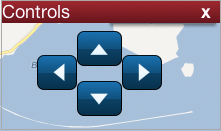
\includegraphics[scale=0.7]{ui/controls.png}
\caption{Controls}
\label{fig:controls}
\end{figure}
By tapping on the upper button, the next image is placed on the map. The right button plays through the simulation automatically. The left and bottom button both do the opposite. Also a pause button stops calling the next or prevImage function out the map object. As previously discussed the controls appear in the right top of the screen. If the user need the controls on the bottom part of the screen, the user can also tap and drag the controls. Because the space of the tablet is limited the user can make the decision of placing the controls somewhere else, note that the controls are constrained to the right side of the screen. The reason is that the controls are meant to be used by the user's right hand.
 
\subsection{Chart Display}
The chart data is the  
 
\section{Scalability}
The server \url{sangkil.science.uva.nl} is tested on scalability. An important part to notice when testing a server is how well it performs concerning how much peers it can serve and how the response time will change if the number of clients increases. By looking at the amount of clients that a server can serve is what scalability stands for. So how do the values change when connections, and therefore client numbers, start to rise.

To test the server, all bottlenecks at client side have to be brought down to a minimum. \url{mangkus.science.uva.nl} is the address of another server with the same specifications. The mangkus server is situated in the same server rack as sangkil. The TCP/IP packages do not have to travel around the world in order to reach the destination, so the response time when not in a stress test could be in optimum state. 

\subsection{Testing}
So testing the sangkil server is done from the server mangkus. A tool siege is used for testing the server, previously discussed in section \ref{sec:scalability} in part one.
\begin{lstlisting}
$ siege -i -b -f file.txt -c $1 -r $2
-i		randomly picking request out of file.txt
-b		no delay between the next request a client does
-c		concurrent processes
-r		number of repetitions
\end{lstlisting}

Testing is done by changing the concurrent processes and keeping the repetitions the same, or the other way around. That way a little grid search can be preformed to find a weakness in the server. The results of this search are discussed in the following sections. 

\subsection{Results and Analysis}
In the first series of tests the repetitions number is the same and the amount of concurrent clients is changed. The amount of concurrency is displayed on the x-axis. Note that it could be that a concurrent value that is tested is not been reached by the server. Concurrency means the amount of clients averagely served by the server for testing at a certain concurrent number. So 500 clients with 10 repetitions could mean that the server does not reach a concurrent level of 500 clients. The reason is that the requests happens so fast that their is no point in time the server handles the full amount of clients that are requesting data.
\begin{figure}[H]
\center
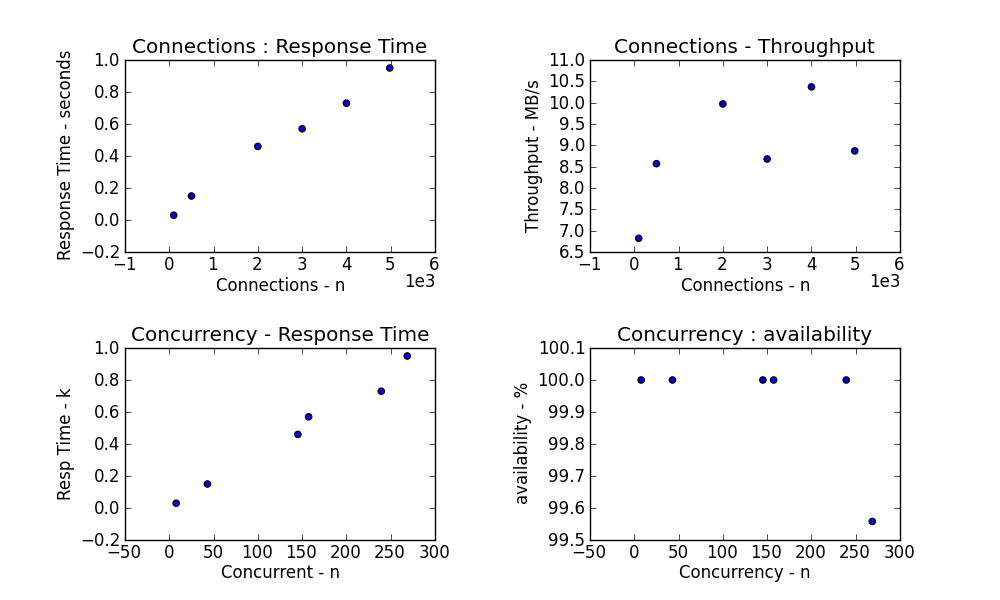
\includegraphics[scale=0.6]{server/siege_10r.png}
\caption{10 repetitions, concurrency 10, 50, 100, 200, 300, 400, 500}
\label{fig:10r}
\end{figure}
See top left graph of figure \ref{fig:10r}. These results suggests that with 10 repetitions and a rising number of concurrent clients the response time increases some what linearly.  100 more clients can be roughly the same as an increase of response time of 0.1/0.2 seconds. 

The throughput (top right figure \ref{fig:10r}) rises when the number of clients rises. This is a good sign when talking about scalability. When the throughput rises when client numbers are rising it means that it can transfer more data when more clients are requesting data. 

The transfer rate is the average number of requests that are handled per second. This rate does increase when more clients are requesting url's but it does not go up linearly.

The availability (right bottom graph) drops when concurrency increases. But it does not drop a lot. That's a positive and negative finding. When the amount of users starts to rise the availability needs to be 100\%. A drop of 0.4\% means that roughly 20 requests ($5000 * 0.004$) out of the 5000 requests in total, would not be answered. 

\vspace{0.5cm}
\begin{figure}[H]
\center
\includegraphics[scale=0.6]{server/siege_50r.png}
\caption{50 repetitions, concurrency 10, 50, 100, 200, 300, 400, 500}
\end{figure}
The same conclusion can be drawn concerning the response time. Notice that the linear increase is roughly the same, but the concurrent clients are now more than the previous test.
The Throughput is higher than the previous test. This means that the server's bandwidth sends more MB/s when more clients are requesting data. It would be interesting to see if this number would climb further.
\begin{figure}[H]
\center
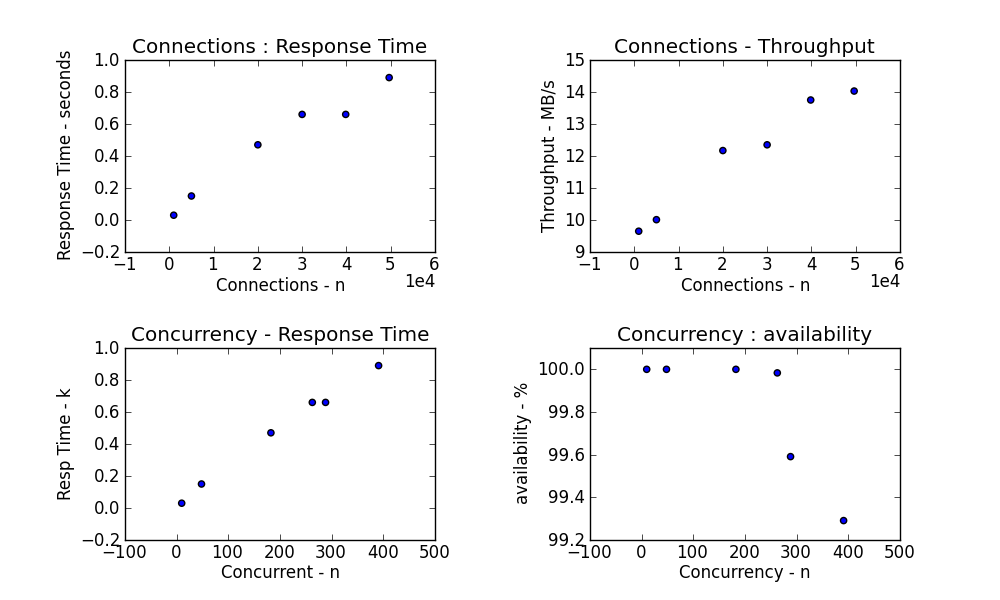
\includegraphics[scale=0.6]{server/siege_100r.png}
\caption{100 repetitions, concurrency 10, 50, 100, 200, 300, 400, 500}
\end{figure}

\begin{figure}[H]
\center
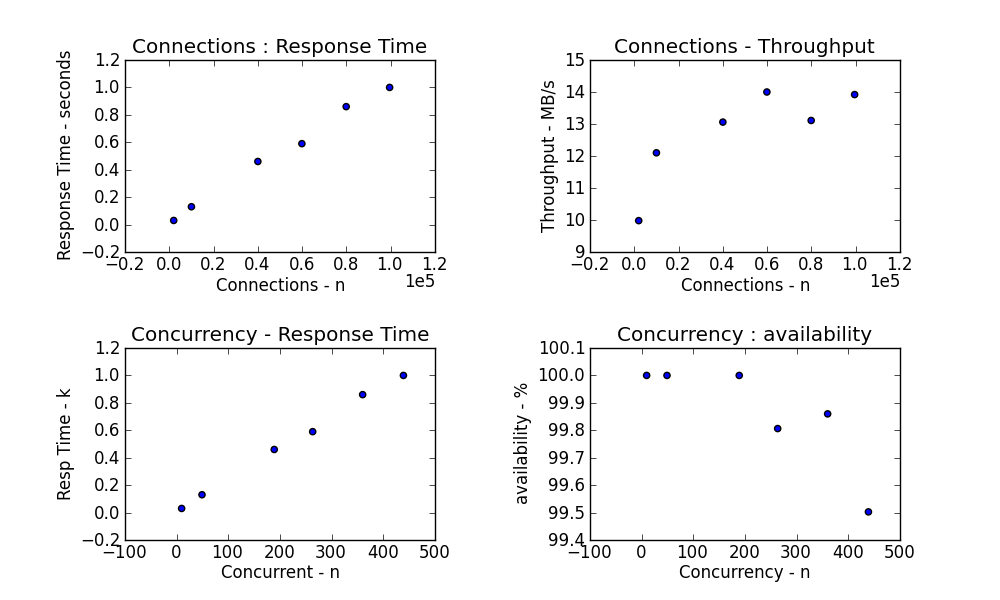
\includegraphics[scale=0.6]{server/siege_200r.png}
\caption{200 repetitions, concurrency 10, 50, 100, 200, 300, 400, 500}
\end{figure}

It does not seem to matter how much repetitions are preformed by a certain number of concurrent clients. This suggests that it could mean that only weak spot of the server concerning the response time depends on how much clients at a time are demanding a request. It looks like it does not matter how much repetitions those clients preform, it has no influence on the response time.
The throughput does rise when the amount of repetitions go up. 



\section{Deployment}
For installing the application to a device the sencha's command line tool is used. In the root folder \texttt{packager.json} can be found. In this file the field for building the application has to changed. See below, listing \ref{lst:packager}.
\begin{lstlisting}[caption={packager.json},label={lst:packager}]
	/**
	 * @cfg {String} platform
	 * @required
	 * This is the platform where you will be running your application.
	 * Available options are:
	 *  - iOSSimulator
	 *  - iOS
	 *  - Android
	 *  - AndroidEmulator
	"platform":"iOS",
\end{lstlisting}
Now by executing the command.
\label{appnative}
\begin{lstlisting}[caption={command to build native},label={lst:buildnative}]
$ sencha app build native
\end{lstlisting}
The application is packaged. All the javascript code's dependencies are resolved, minified and placed in the \texttt{build} folder. The \texttt{build} contains two folders. One \texttt{package} and one \texttt{native} folder. In the \texttt{package} folder the developer can see what result of the minification is, and can also test in the browser if everything still works. The native files are placed in the \texttt{native} folder. When executing for Android the applications extension will be a .apk\todo{ref to apk?}, for iOS it will be a .app file.  The file can be transferred to the device and installed. On Android it's easier that iOS. When building for Android the result of the command(listing \ref{lst:buildnative}) runs the application when done with packaging. When building for iOS, sencha creates a .app file that can be transferred to the device by itunes\footnote{How to do this can be found in the video ``Getting started'' at: \url{http://docs.sencha.com/touch/2-0/\#!/guide/getting\_started}}.

The deployment can be distributed to other devices. On Android devices it's possible to install .apk files apart from the Market / Play Store. For iOS this is more difficult. When a developer is in the possession of an Apple's developer account the UUID(Unique Identifier) needs to be added to the provisioning portal. This grants the device to install applications that are also registered by the developers account. \todo{apple provisioning}.

\section{Does Sencha Touch suffice}
Sencha Touch 2 is used in this project for the cross-platform capabilities. One of the research question was to find the best tool to meet the requirement of cross-platform. Let's start with the fact that everything works both on a Asus tf300t Transformer Pad with Android , iPad 2 with iOS 5.1.1 and the browsers Safari and Chrome. Installing an application to the device involves For testing this application on the iPad 2 jailbreaking had to take place. How to jailbreak the iPad to is desribed here \url{http://greenpois0n.com/}. For enabling tp install without a developers account apps without ``Appsync'' has to be installed.\footnote{\url{http://www.ijailbreak.com/cydia/install-cracked-apps-ios-5-0-1-with-appsync-installous/}}



\section{Conclusion}

\section{Discussion}
Future research:
small screenshots with map
a lot of data


\newpage
\bibliographystyle{plain}
\bibliography{references}
\newpage
\appendix
\section{Area API}
\label{sec: area_api}
\begin{lstlisting}
# Terms

Map: digital terrain map (DTM)
Projected map: inundation map projected/transformed to WGS84/EPSG:3857
               (e.g. Google Maps) projection system

# Area List

GET /area/list.json

response:

    {"stat": "ok",
     "areas": [
        {"area_id": 1,
         "name": "Science Park",
         "center": [52.347185, 4.9370885],
         "corners": [[52.334349, 4.904065], [52.334349, 4.970112],
                     [52.360021, 4.970112], [52.360021, 4.904065]],
         "visbounds": [52.360021000000003, 4.9701120000000003,
                       52.334349000000003, 4.9040650000000001]}

     ]}

note:

    - "center" is the center point coordinate of the map, in latitude
      and longitude
    - "corners" contains 4 pairs of numbers showing the WGS84 coordinate of the
      four corners of the area, in latitude and longitude
    - coordinates in the "corners" correspond to the coordinate of
      the lower left, lower right, upper right, and upper left corners
      of the area, consecutively
    - "visbounds" contains 4 numbers representing the WGS84 coordinate of
      north, east, south, west in latitude or longitude for laying out the
      projected flooding image


# Area List (query)

GET /area/list.json?bounds=north,east,south,west



# Area Info

GET /area/<area_id>/info.json

response:

    {"stat": "ok",
     "area_id": 1,
     "name": "Science Park",
     "center": [52.347185, 4.9370885],
     "corners": [[52.334349, 4.904065], [52.334349, 4.970112],
                 [52.360021, 4.970112], [52.360021, 4.904065]],
     "size": [880, 565],
     "extents": [[0, 0], [0, 0]],
     "projection": "...",
     "visbounds": [52.360021000000003, 4.9701120000000003,
                   52.334349000000003, 4.9040650000000001],
     "vissize": [880, 565],
     "dikes": [[[lat1, lng1], [lat2, lng2], [lat3, lng3], [lat4, lng4]],
               [[lat5, lng5], [lat6, lng6], [lat7, lng7], [lat8, lng8]]]
    }

note:

    - "corners" contains 4 pairs of numbers showing the WGS84 coordinate of
      the four corners of the area in latitude and longitude
    - "size" shows width and height of the DTM and Inudation Zones Map
    - "center" is the center point WGS84 coordinate of the map, in latitude
      and longitude
    - "extents" contains 2 pairs of numbers showing the coordinate of
      the lower left and upper right corner of the map in its original
      projection unit
    - "projection" contains projection parameter of the map in WKT format
    - "visbounds" contains 4 numbers representing the WGS84 coordinate of
      north, east, south, west in latitude or longitude for laying out the
      projected flooding image in this area
    - "vissize" is the size of projected flooding image in this area.
      Because of the projection, the flooding image may have different size
      compared to the original DTM/Inundation Zones size
    - "dikes" contains a list of closed polygons described by a list of
      WGS84 coordinates which shows the region of the dikes in the area

# Digital Terrain Map

GET /area/<area_id>/topography.txt
GET /area/<area_id>/topography.txt.gz


# Inundation Zones Map

GET /area/<area_id>/zones.txt
GET /area/<area_id>/zones.txt.gz

# Coordinate to Inundation Zone id mapping

GET /area/<area_id>/izid.json?latlng=<LAT>,<LNG>

response:

    {"stat": "ok",
     "area_id": 1,
     "latlng": [52.347185, 4.9370885],
     "izid": 12345}
\end{lstlisting}
\newpage
\include{lsm-api}
\newpage
\include{drfsm-api}
\end{document}